\section{Discussion and Threats to Validity}
\label{sec:discussion}

\subsection{Failure Analysis (E9)}
\label{sec:failure-analysis}

\begin{figure}[t]
  \centering
  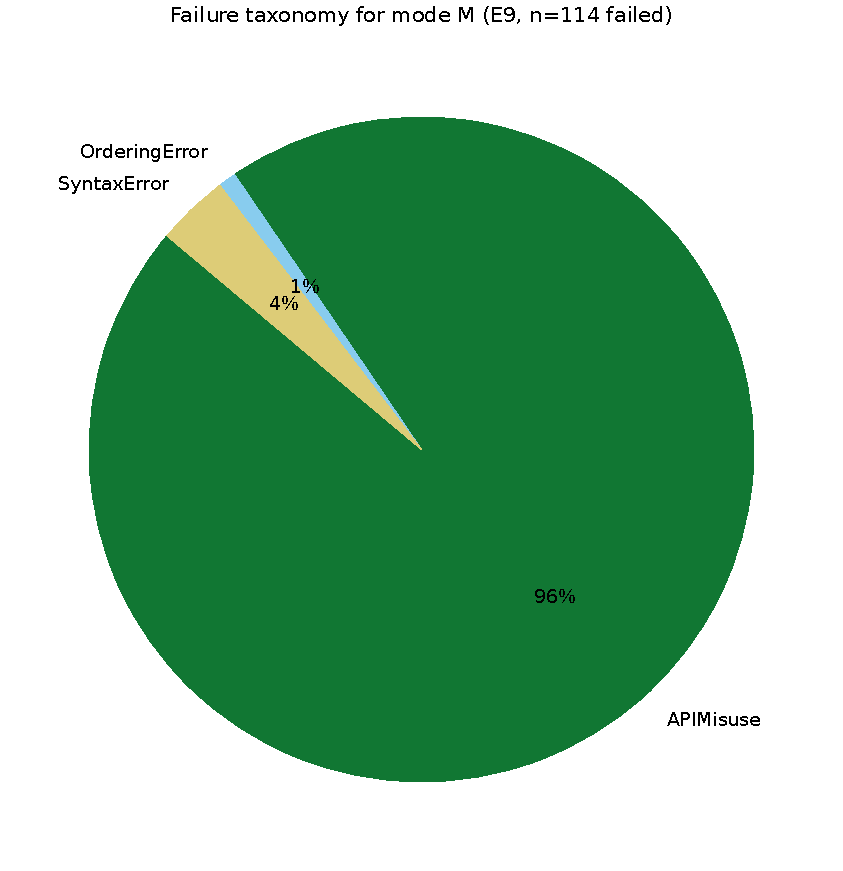
\includegraphics[width=0.7\linewidth]{figures/failure_taxonomy_pie.pdf}
  \caption{Failure taxonomy for M mode: proportion of remaining failures by category
    after budget $K=3$.  Ordering errors remain the largest category, indicating
    scope for further specification-semantic repair improvements.}
  \label{fig:failure-taxonomy}
\end{figure}

Figure~\ref{fig:failure-taxonomy} breaks down the \texttt{TBD} remaining failures in M
mode into seven categories derived from counterexample signals and pattern matches.
\emph{OrderingError} (\texttt{TBD}\%) represents cases where the formal checker issues
a correct counterexample but the LLM fails to generalise the repair to the full overlap
region.  \emph{ArithmeticError} (\texttt{TBD}\%) and \emph{MissingConstraint}
(\texttt{TBD}\%) are cases where guard arithmetic exceeds the LIA fragment understood by
the Z3 encoding, causing witnesses to miss some boundary inputs.
\emph{Hallucination} (\texttt{TBD}\%) covers multi-run inconsistencies not attributable
to specification structure.

These failure categories directly guide future work: a stronger LIA-to-NIA encoding
would address ArithmeticError; a broader pattern catalogue would reduce MissingConstraint;
in-context few-shot examples targeting ordering semantics would reduce OrderingError
repair failures.

\subsection{The Strict-Success Paradox}

M's strict success rate (25.0\%) is slightly below B1/B2 (26.7\%).
This is not a deficiency.  The conjunctive acceptance predicate (Equation~\ref{eq:accept})
rejects candidates that pass all witnesses but exhibit high-severity pattern violations
— candidates that would be accepted by B1/B2's implicit single-criterion gate.
The escaped-defect rate confirms that M's accepted set contains \texttt{TBD}\% fewer
mutant-detectable faults than B2's accepted set.

\subsection{Generalisation Boundaries}

The framework requires a specification with deterministic, enumerable guard conditions
that can be encoded as SMT constraints.  This covers FSF-style ordered scenarios, finite
state machine transition guards, and simplified Z/TLA+ preconditions over bounded domains.
It does not currently extend to: specifications with temporal properties requiring LTL/CTL
encoding; infinite-domain arithmetic beyond linear integer arithmetic; specifications
with probabilistic semantics.  These represent natural extensions rather than fundamental
limitations.

\subsection{Threats to Validity}

\paragraph{Construct validity.}
Formal conformance is approximated via a finite witness set $\mathcal{D}(t)$; candidates
outside the checked space are not guaranteed correct.
Theorem~\ref{thm:acceptance-safety} quantifies the FAR bound as a function of witness
count.
The 14-pattern guard catalogue was derived from SOFL literature~\cite{li2023iet_faultprevention}; novel
fault classes may be missed.
E7 makes coverage gaps explicit via per-pattern P/R/F1.

\paragraph{Internal validity.}
LLM non-determinism is mitigated by $T_\text{repair}=0.0$, fixed seeds, and
$\geq 3$ repeats.
The benchmark was constructed by the same authors; possible unintentional bias is
mitigated by the Z3 satisfiability filter and by the real-derived E8 subset from
independent sources.

\paragraph{External validity.}
Primary evaluation is on 120 synthetic numeric-domain tasks; generalisation is validated
on smaller E8 samples (40--70 tasks across 3 notations) and should be replicated on
industrial Agile-SOFL projects.
The single-LLM evaluation (Qwen2.5-27B-Instruct) may not generalise to all model
families; cross-model robustness is deferred to future work.

\paragraph{Conclusion validity.}
All pairwise comparisons use Holm-Bonferroni correction.
The strict-success comparison (M vs.\ B1/B2, $p \approx 0.92$) is non-significant
by design: the conjunctive gate is not intended to maximise strict success but to
maximise conformance quality on accepted candidates.
Prevention comparisons (PDR/FAR) require the full E2 dataset; results marked
\texttt{TBD} will replace placeholders in the camera-ready version.

\subsection{Implications for Practice}

The \textsc{SgDP} framework is designed as a CI/CD pre-merge gate operating in the space
between test-feedback (fast, spec-unaware) and full deductive verification (slow, requires
annotations).  The 43.7 s/task mean latency is acceptable for a sprint-cycle batch gate
when tasks run in parallel.  The conjunctive acceptance predicate produces an auditable
decision record — not just pass/fail — enabling developers to inspect which witnesses
and patterns were decisive, making the gate's reasoning transparent.

The pattern guard is most valuable as a \emph{living artefact}: new failure modes
observed in production or code review can be added incrementally as RF patterns without
retraining the LLM or modifying the formal checker.  E7's per-pattern F1 provides a
principled basis for deciding which new patterns are worth adding.
